\subsection{Steered MD Transit Simulations}

\subsubsection {\suldiox~Orientation}

	The orientation of \suldiox~molecules throughout the aqueous adsorption process was monitored during the transit SMD simulations. The angles $\theta$ and $\phi$ of the transiting \suldiox~(Figure \ref{fig:water-angles}) were calculated for each timestep of the SMD simulations as the \suldiox~was pulled into the water slab from the gas phase, both in the neat-water and saturated slab systems. The orientation depth-profiles were collected for the 50 simulations of both systems for various distances from the water surface location, resulting in the 2-dimensional angle and depth-profile histograms shown in Figure \ref{fig:so2-transit-angles}.

\begin{figure}[h!]
	\begin{center}
		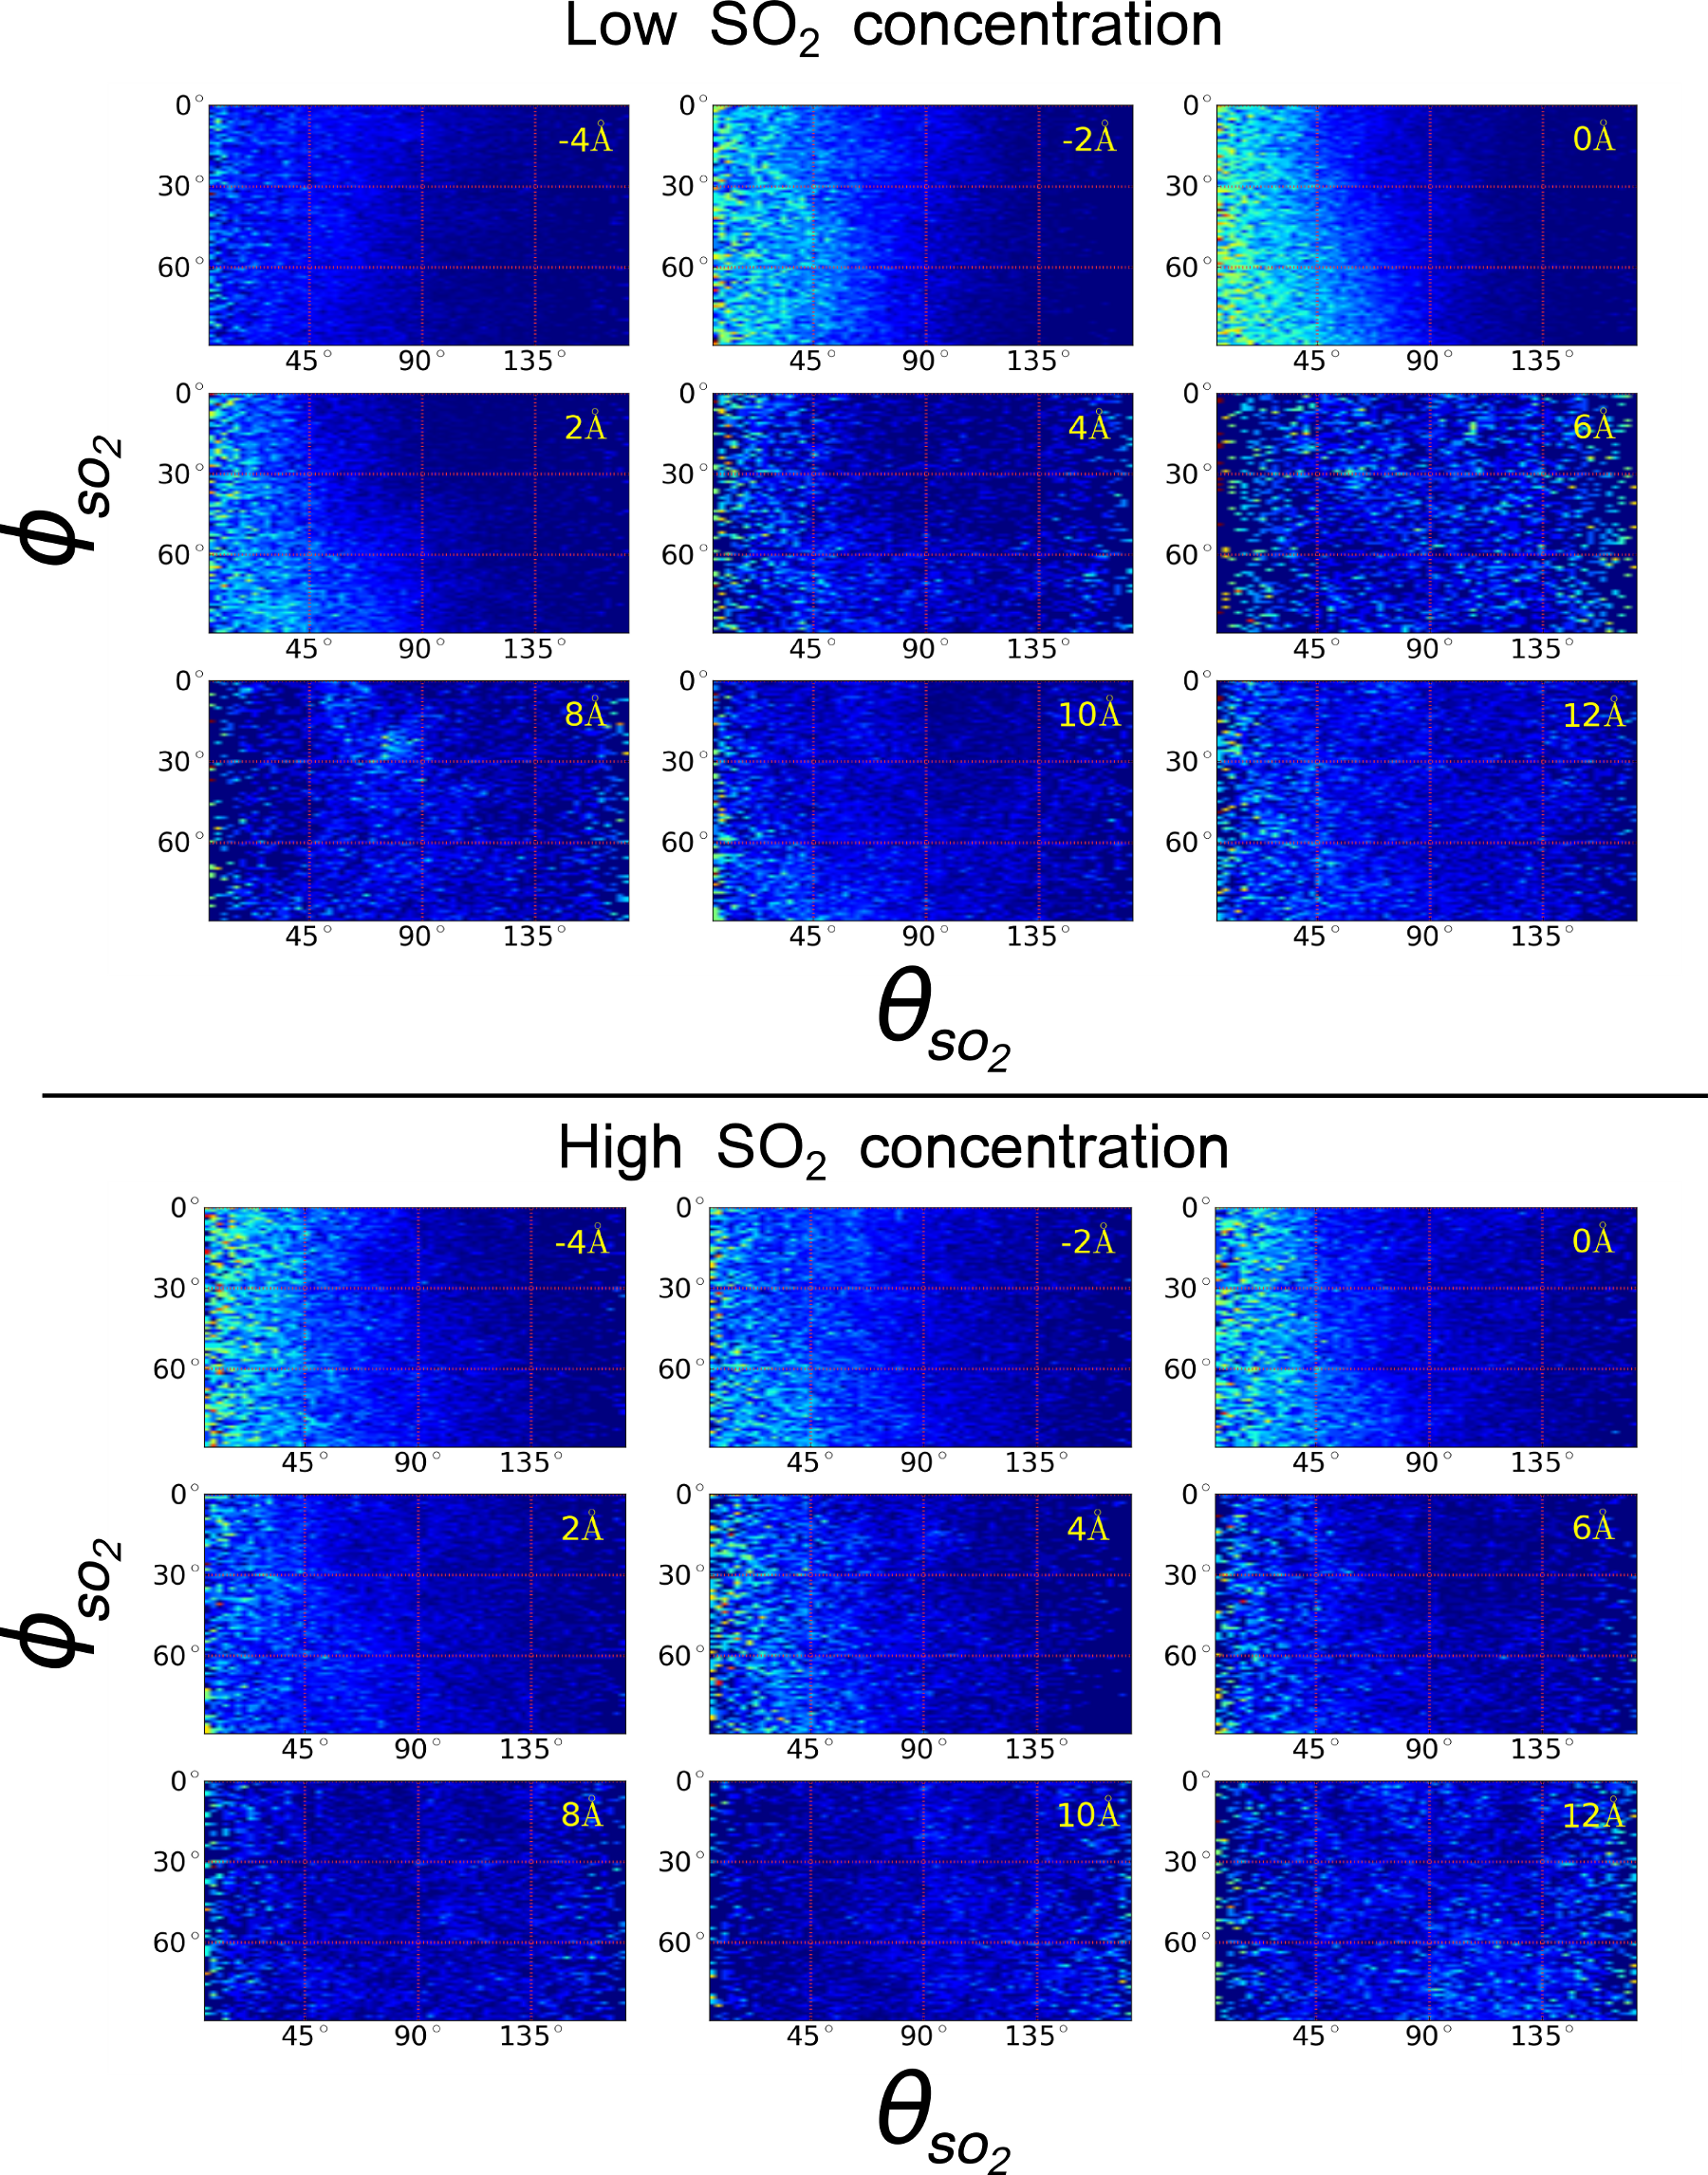
\includegraphics[scale=1.0]{images/so2-angles/theta-phi-transit.png}
		\caption{Molecular orientation distributions of an \suldiox~at different interfacial depths of an aqueous slab during SMD transit simulations. Both the neat-water (top) and saturated (bottom) data sets were analyzed to determine the angles $\theta$ (horizontal axes) and $\phi$ (vertical axes) of the transiting \suldiox. The distributions shown are those for the single transiting \suldiox~molecule averaged over the 50 SMD simulations.}
		\label{fig:so2-transit-angles}
	\end{center}
\end{figure}

	From its starting position above the water surface, until the \suldiox~moves to within 6\angs~of the water surface location of both systems, the orientation is isotropic in $\theta$ and $\phi$. Isotropic orientation is manifested in the plots as mostly uniform coloration at a given distance from the surface independent of $\theta$ or $\phi$. Near and into the interfacial region the bisector angle $\theta$ becomes more perpendicular to the water surface ($\theta \approx 0$\textdegree) with the \suldiox~sulfur pointing into the water phase, consistent with the equilibrium MD simulation results above. At the point when the \suldiox~reaches the water surface location (0\angs), the bisector is perpendicular to the interface in both the neat-water and saturated systems. %Figure \ref{fig:so2-surface-angles}a depicts \suldiox~near the water surface with the bisector aligned perpendicular to the interface. 
	In the absence of simulated ionic species that form through \suldiox-\wat~chemistry at the surface, it is clear that the adsorbing \suldiox~in the gas phase takes on a preferred orientation to adsorb on a water surface. The main difference between the neat and saturated water systems is where the point of the transition from isotropic to preferred orientations is found. 
 
  % theta differences
  Comparing in more detail the difference in these two systems upon \suldiox~approach, for the neat-water surface, a transition occurs at approximately 4\angs~above the surface water location. Below 4\angs~above the surface, \suldiox~has a preferred net orientation and is close enough to the water surface that it begins to interact with the topmost surface waters. In the saturated system, the same trend occurs, however the onset of the perpendicular orientation begins at approximately 8\angs~above the surface. The layer of adsorbed \suldiox~already present in the saturated system most likely interacts with the transiting \suldiox~molecule. Also, topmost water molecules from the surface move up to a few \angs~inside the adsorbed \suldiox~layer and interact with the transiting \suldiox~further from the surface than those in the neat-water system. It is remarkable that the orientational trend appears so strongly in the $\theta$ plots even with so little data as was collected from the single \suldiox~molecule of each simulation. From onset of orientation above the surface until 10\angs~below (not shown), the \suldiox~holds a preferred orientation.

%\begin{figure}[h!]
	%\begin{center}
		%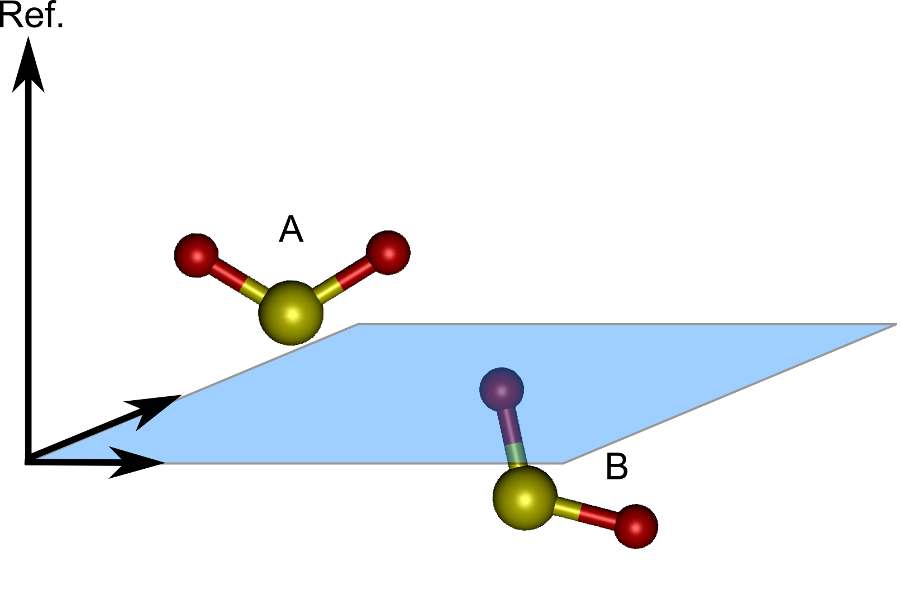
\includegraphics[scale=1.0]{images/angle-cartoons/so2-surface.png}
		%\caption{(A) \suldiox~molecules above and below both neat-water and saturated water surface location orient with the bisectors perpendicular to the interface. The \suldiox~sulfur points down towards the aqueous phase. (B) In the neat-water system, a transiting \suldiox~molecule located below the water surface briefly reorients with one S-O bond more towards the interface above, and the other bond pointing further down into the water bulk.}
		%\label{fig:so2-surface-angles}
	%\end{center}
%\end{figure}

  % phi differences
	%Indeed, the $\phi$ orientations appear mostly isotropic without any clear trends for preferred orientation in that angle. This appears as a mostly uniform color across the entire plot, with minor variations that are disjointed throughout the distance range.

 With a mostly perpendicular bisector angle, it is expected that the values of $\phi$ for \suldiox~would be isotropic relative to the reference axis. This is the case in both systems, with only a few exceptions. In both systems the $\phi$ profiles exhibit mostly isotropic distributions above 0\angs, with several regions of lighter coloration interspersed, but without a clearly formed orientational trend. At the neat-water surface and just above (from 0-2\angs~above the water phase), the $\theta$ profile broadens to $\theta = 90$\textdegree, near $\phi = 90$\textdegree~appearing as a shoulder of light coloration in the bottom-left of the 0-2\angs~axes. This indicates that \suldiox~inclined up to 90\textdegree~from the surface normal will have a preferred $\phi$ orientation lying more flat to the water surface. This is in contrast to \suldiox~molecules above the water surface location, oriented more perpendicularly and without a preference for a particular range of values in $\phi$. The behavior is likely due to the interaction between the waters and the S-O bonds leading to a higher solvation than above the water surface location. As the \suldiox~is solvated by more highly-coordinated bulk water, the S-O bonds experience less equal interaction environments. Baer et al. noted that their force field model for the \suldiox~does not reproduce well the first hydration shell geometries,\cite{Baer2010} so conclusions regarding the specific interactions and hydrate geometries between the \suldiox~and \wat~cannot be made here. It is notable that the same reorientation does not occur as strongly in the saturated system. The presence of the adsorbed \suldiox~layer apparently decreases the reorienting behavior likely because of the disrupting effect the higher \suldiox~concentration has on the water interactions in the interfacial region. %Below this 5\angs~region under the surface, the \suldiox~resumes an isotropic orientation as it becomes fully solvated by bulk waters.

  %Upon approaching the saturated surface at approx. 5\angs, the \suldiox~$\phi$ orientation distribution begins to cluster near $\cos(\phi)=1$, with the $\theta$ distribution remaining more isotropic, but with a trend of $\cos(\theta)>0$. At 5\angs the \suldiox~begins interacting with the other \suldiox~molecules that sit atop the water, and the resulting orientation distribution suggests that contact with the \suldiox~layer causes the adsorbing molecule to lie more flat to the surface. Within this same region from 0-5\angs above the surface, the $\phi$ distribution of the neat-\wat~system remains isotropic. The intensity of the distribution (darker blue) also indicates that the \suldiox~spends little time in this region, as it is quickly adsorbed further into the water bulk.

	%Just below the water surface as the distance moves into negative values, both systems show clear orientational preferences. In both systems the bisector orientation clusters such that $\cos(\theta)<0.5$, with most of the distribution intensity around $\cos(\theta)=1$. This suggests that \suldiox~in a water surface orients with the sulfur pointing into the water bulk, and the oxygens pointing towards the surface water molecules.

	%Differences ocurr between the system orientation profiles once the \suldiox~has moved further than 10\angs below the surface. While both $\theta$ and $\phi$ hold the same trend from just under the surface through to the bulk of the slab in the saturated system, the orientation profile becomes much more isotropic past 10\angs under the surface of the neat-\wat~system. The orientation effect is shallower under the neat-\wat~surface. However, the orientation distribution peaks most intensely, and more tightly clustered with the \suldiox~bisector aligning with the surface normal, just underneath the neat-\wat~surface than the saturated one. The distributions thus show an orienting force extending deeper into the surface of the saturated system than the neat-\wat~system. In terms of how deeply the \suldiox~molecule is oriented, the interfacial region of the saturated system is larger and extends further into the aqueous bulk.
